\section{State of the art}

\subsection{Plant as sensor}

\subsubsection{Human-Plant cohabitation}

Plants have a lot of benefic effects on human. The study from Charles Hall and Melinda Knuth \cite{hallUpdateLiteratureSupporting2019}
explain all the benefits of plants on our human system.
Watts and al. shows that urban "greening" (add green spaces in urban city)
increase tranquility, relieve stress and anxiety \cite{wattsEffectsGreeningUrban2017}.
An experience has been conducted in offices by Ikei and al \cite{ikeiPhysiologicalPsychologicalRelaxing2014}
to expose roses to employees. The experience showed that the "parasympathetic nervous activity was significantly higher while viewing the rose". 
The subjects were more comfortable
being expose to roses than people that were not.

On top of that, we, as human, are spending 85\% of our live indoor \cite{leeInteractionIndoorPlants2015}. We are subject to the
\textit{technostress}. \textit{Technostress} is a term introduced by Brod and Craig \cite{brod1984technostress} in 1984.
Brod and Craig describe it as a modern disease caused by the inability of a person to interact and use information and communication technologies
in a healthy way \cite{ayyagariTechnostressTechnologicalAntecedents2011}. Lee and al \cite{leeInteractionIndoorPlants2015} compared 
the stress caused by the doing a task on a computer to interacting with a plant (specifically transplanting it).
The computer task was increasing the level of stress (increased diastolic blood pressure and sympathetic nervous system activity for example).
The plant interaction on the other side was found to create positive feeling to the subjects. The plant is a good way of reducing
the \textit{technostress}.

Another study comes to the same conclusions. Hassan and al. \cite{hassanEffectsPlantActivity2018}
studied the effect of plant interaction on young adults subjects to 
stress induced by electronic devices (similar to \textit{technostress}).
They concluded that significant differences in blood pressure occurred
between the subjects interacting with a plant (transplanting) and the 
one that add to do the task on the electronic device (phone).

It's understandable that people see plants as un-stressful and not harmful. This makes them a perfect human-machine interface.
% Make plants the perfect interface, not harmful, enhance the link

\subsubsection{Human-Plant interaction}

The human plant interaction has been studied. Seow and al. \cite{seowPudicaFrameworkDesigning2022}
created a framework that is able to detect when something (and someone) interact with a plant.
However, this is not any plant, the plant used is the \textit{Mimosa Pudica}. This plant is special,
when something touches its leaves, the plant closes its leaves to protect them from the danger \cite{volkovMimosaPudicaElectrical2010}. 
An electrical impulse is released and is catch by the device Seow and al. developed. The electrical 
signal is easy to catch and thus can be used as actuator. However, the plant needs time and energy
to re-open the leaves. This framework also can't be generalized to other species of plants.

\begin{figure}[h!]
    \centering
    \includegraphics[width=0.8\textwidth]{pudica_framework.png}
    \caption{\textit{Pudica framework} made by Seow and al. The \textit{Mimosa Pudica} is a
    special plant that react to the interaction by closing its leaves. The framework
    captures the electrical impulse and then interprets that an interaction happened.} 
    \vspace{0.1cm}
    \label{fig:pudica_framework}
\end{figure}

Sato and al. used the process of capacitive sensing to detect interaction with objects of our daily lives \cite{satoToucheEnhancingTouch2012}.
In this paper, they proposed a device called \textit{Touché} that use swept frequency capacitive sensing  to detect touch interaction 
but also more complex interactions (such as interacting with a finger, the whole hand...). More complex 
interactions are captured using machine learning algorithm.

This paper doesn't apply the device to plants. Poupyrev and al. \cite{poupyrevBotanicusInteracticusInteractive2012}
used the device on plant to demonstrate the usage. This swept frequency technique is usable and better
than the previous single frequency technique as it captures more data.
In their article, Honigman and al. \cite{honigmanTechniquesSweptFrequencyb} adapted the \textit{Touché}
device to be use with an Arduino\footnote{Open source compute unit} microcontroller. This allowing people
to reproduce the set-up easily.


\subsubsection{Plant as sensors Plant transformed into sensors}

\subsubsection{Touch sensors}

Usual sensors uses physical properties to capture the data. For instance, in 1999, Hinckley and al. \cite{hinckleyTouchsensingInputDevices1999} 
were building a touch sensor made of conductive paint. The conductive paint is used as an electrode.
In the circuit, a component is generating a 30 Hertz square signal. When the user interact with the conductive surface,
it shifts and induce delay in the square wave. The delay induce by the user hands is caused by its natural
capacitance. This circuit, however, gives a boolean output based on a threshold. The answer is \textit{touched}
or \textit{untouched}. % Evoke the "The present work has demonstrated that touch-sensing is an
% orthogonal property of input devices that does not
% necessarily have to be coupled with position sensing

When thinking of touch sensors, we think about the trackpad/touchpad that we daily use in our personal 
computer. Those sensors use resistive or capacitive sensing. Both of these techniques are based on electrical
properties. Resistive sensing is based on the perturbation of the resistance in a circuit. Whereas 
capacitive is based on the capacitance. Capturing those specific properties are usually the basic of 
touch sensors.

For instance, Olberding and al. created a cuttable multitouch sensor based on capacitive sensor \cite{olberdingCuttableMultitouchSensor2013}.
This specific sensor allows to create something similar to a trackpad but with different shapes.

Reading the capacitance at a fixed frequency is working and is already used in our daily lives. 
However, to capture more complex interaction and to rely on the data, adding another dimension of data is useful.
Swept Frequency Capacitive sensing consists on emitting a electrical signal and then read the capacitive values
similar to what a classic sensor would do. However, the electrical signal is not generated at a fix frequency
but is generated following a changing frequency. 
Sato and al. introduced first this technique in the \texit{touché} device \cite{satoToucheEnhancingTouch2012}.
This allows to get richer information on the output of the device. \textit{Touché} allows then to capture 
the information on a variety and a multitude of daily objects.
Indeed, searching through many frequencies make it simpler to find small changes and though different kind and type 
of interactions.

\subsubsection{Sonification}

Sonification is “the use of non-speech audio to convey information or perceptualize data” \cite{hermannListenYourData}.

The sonification has been used for a long time using the human ear sensor to interpret data. For instance, the Geiger 
counter is using the sonification to measure the ionizing radiation. This sensor is "beeping" and "crackling"
depending of the level of radiation.

Herman and al \cite{hermannListenYourData} created two sonification models to represent particles moving. They are 
saying that the sonification is allowing a multidimensional representation of the data captured.
Humans are sensible to sounds. The sound allows a "rapid screening" because it is easier to listen to a sound than
read a graph or a text. The sound when combined with visualization is bringing more granularity and understanding.
They are also adding that we are using sound to diagnosis issues on a daily basis ; giving the example of a car
mechanic that is having a failure and that we can predict.

The sonification has been used in many projects. Ballora and al. \cite{ballora2012use} designed a project that mix the fluctuation of the stock
market with the apparition of keyword on Twitter social network. They were mapping specific and defined keyword with specific
sounds. The designed an app to be able to tweak and change the volume of the different sounds. The same procedure 
is applied to the variation of the stock price.
They conducted this experiment in order to add another possible channel of information in the market place.
The traders and people working there are already flooded with visual information. This new channel could allow to 
process more data.
The result were encouraging. However, this experiment rose issues. People were annoyed and disturbed by the sound.
They were lowering the volume and thus not hearing it. Some other people were just too much concentrated on 
their task that they did not hear the variations.
More experiment should be conducted to refine the sound created and the level needed.

In the same direction, Ballora and al. \cite{ballora2012use} also developed a device to monitor the heart rate of people
using sonification. It takes the output of an electrocardiogram and transform it into a sound. Each of the ECG's frequencies
were pass into a filter and then given a specific sound.  
The output of the sound creation is then listened to and interpreted. This application with a trained ear can help
diagnosis the sleep apnea through heart variability.


\subsubsection{Sonification on microcontrollers}

MCUs\footnote{microcontrollers} \cite{rochim2019design} is a kind of small computer.
Those devices can be used to generate sound. The most common way of doing electronical music
is to use MIDI\footnote{Musical Instrument Digital Interface} \cite{loyMusiciansMakeStandard1985}.
MIDI has been created in order to create music with digital computer. MIDI do not describe directly 
the audio signal but the human actions to create the signal (such as turn the knob left, push the slider...).
MCU are able to produce those kind of directives \cite{fazendaProceedingsInternationalConference1}\cite{fazendaProceedingsInternationalConference2}.
However, the MCU can produce MIDI but MIDI does not directly generate sounds. A synthetizer is needed to create the sound
described.

For our use case of embedding the device, we look at MCU that were able to directly generate the signal 
from a DAC\footnote{Digital to Analog Converter}. Projects had been conducted with many microcontrollers such as a small
8 bits AVR microcontrollers (ATmega32) \cite{hussainAVRMicrocontrollerImplementation2011}. This paper does not include limitation of
such a product but we can guess that the 8 bits microcontroller is limiting the sound quality. A larger project from Shaer and al.
\cite{shaerInteractiveCapacitiveTouch2020} is including an Arduino Mega controlling the visual effect of the project,
but also the interaction sensors. The Arduino Mega is then sending MIDI information to Teensy 3.2. The Teensy is then 
generating the sound. The project is still too large to be fully embedded but the Teensy 3.2 is a promising compute unit.
The Teensy 3.2 is running at 72 MHz, way faster than the ATmega32 that is operating at 16MHz. The frequency is essential
when trying the produce sound signals.


\subsubsection{Commercial products}

Generating music from plants is not a new concept. Several commercial products are available on the market.
Looking at \textit{PlantWave} device from the eponym company, the device is able to generate sound from the plant. The device is
built using a small box with two electrodes. The electrodes are then connected to the plant. The device generates sound.
The process of sonification is not described and thus is blurry as it is a patent technology. The device is also not open-source

\begin{figure}[h!]
    \centering
    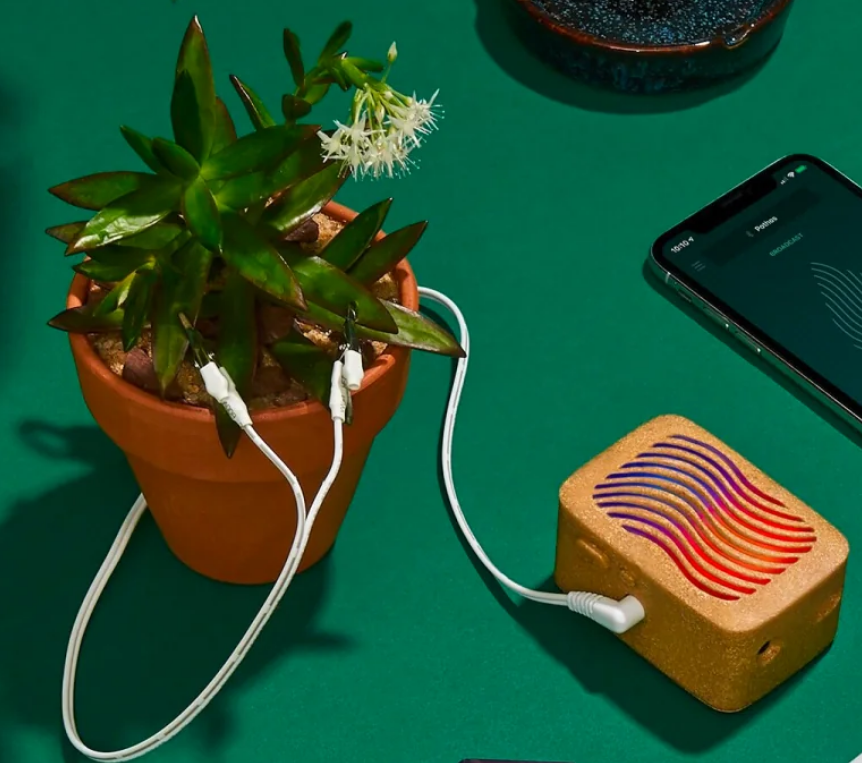
\includegraphics[width=0.8\textwidth]{images/plant_wave_product.png}
    \caption{The PlantWave product on a demonstration picture (source from their website)} 
    \vspace{0.1cm}
    \label{fig:plant_wave_product}
\end{figure}

Another commercial product is the \textit{Music of the Plants} product. How the product works is even more opaque and the company building the product
is sometimes associated with cult and esotericism. The product is also not open-source.


\subsection{Internet of Plants}

The Internet of Plants in not a new word. Nevertheless, the term is not that spread around.
Aliev and al. \cite{alievInternetPlantsApplication2018} evoked the word. The paper explain that
the word is based on the IoT\footnote{Internet of Things}. The paper is using this word 
to describe a system of sensors to monitor plants and crops. This is really close to the IoT
as it is using silicon made sensor to retrieve the data from the plants.

Internet of Plants is especially used for agriculture. In the paper of Steeneken and al.
\cite{steenekenSensorsAgricultureInternet2023}, they are explaining that the use of specific
sensors could and should be very efficient to boost the productivity of the crops.
The paper is also using talking about classic connected sensors but applied to plants.

Like the previous authors, Kitano and al. \cite{kitanoInternetPlantsIoP2022} also used 
this specific word for sensor connected agriculture. I think that the IoP of plants in 
that use is more a specific application of the IoT instead of a specific field of research.

\subsubsection{Distributed system}

The Internet of Plants relies on the paradigm of \textit{distributed systems}. Van and al. define
distributed systems as " collection of autonomous computing elements that appears to its users as a single coherent system."
\cite{steenDistributedSystems2017}. 
Distributed systems scaled up with the improvement of computation power and networking link speed.
It is now possible using networking to spread calculation power around a room or even the world and to
rely on this computation power as a part of a working system.

Even if distributed systems spread up thanks to the increasing networking speed, they are far
from being new.
In 1985 Kleinrock and Leonard \cite{kleinrockDistributedSystems} already
explained the principle of distributed systems. They get inspired by nature looking at bees that are communicating to fetch food,
ants are also communicating but adding also their strength to get back the food.
At this time, adding computation power was a really interesting way of expanding the power on a local network.

Distributed system complicates the monitoring of the system and add complexities and faulty points in the system.
There have been a lot of
research about the best way of linking pieces of a distributed system. Distributed system are usually based on a 
communication protocol such as the internet protocol (IP), bluetooth mesh or even Lora.
Relying on those already existing communication protocol ease the deployment of the application.
However, congested communication protocol or distance can introduce latencies and thus data failure and inconsistency.
It is important in a final product that the data is checked and verified.
We are them introducing the CAP (consistency, availability and partition tolerance) theorem also called Brewer theorem.
It has been introduced by Brewer in 2000 \cite{brewerRobustDistributedSystems2000}.
This theorem explains that it is impossible to have full data consistency, complete availability and partition tolerance
in a distributed system. Only two of the three capabilities can be achieved.
You always have to think about the balance and what is the most important in your system.
It was mainly thought especially for the distributed databases but can also be used for all the distributed systems that are
including a network communication.

On the monitoring side, Joyce and al. \cite{joyceMonitoringDistributedSystems} explained how to build a monitoring
on a distributed system. Monitoring in the case of a full solution is mandatory to be able to capture and react to eventual
failure on the system.

% Adding a new part of the distributed system
%Upgrade the computation power.
% A distributed system is a network of independent computers that work together to achieve a common goal, appearing to users as a single, cohesive system. 
% These computers, often referred to as nodes, share 
% resources, coordinate their activities, and communicate with each other over a network. 
% Distributed systems offer several advantages, such as scalability, fault tolerance, and 
% resource sharing, making them suitable for large-scale applications like cloud computing, 
% databases, and distributed file systems. However, they also introduce complexities, such as 
% handling failures, ensuring data consistency, and managing synchronization across the system. 
% Common challenges include overcoming network latency, ensuring security, and maintaining a balance between consistency, availability,
% and partition tolerance, as described by the CAP theorem.

\subsubsection{Distributed instruments}



\subsubsection{Sonification using software}